% Classe usada para fazer slides
\documentclass{beamer}

% Tema para o template
\usetheme{Goettingen}

% hue br
\usepackage[utf8]{inputenc}
\usepackage[T1]{fontenc}
\usepackage[brazil]{babel}

% para highlight de sintaxe dos codigos
\usepackage{listingsutf8}
% para modificar a cor de fundo de codigos
\usepackage{color}

% cor personalizada para fundo dos codigos - add por jorge
\definecolor{light-gray}{gray}{0.95} %the shade of grey that stack exchange uses

% para usar o lstlistings com os comandos
\lstset{
    %basicstyle=\ttfamily,
    basicstyle=\ttfamily\scriptsize,
    %keywordstyle=\color{blue},
    %stringstyle=\color{green},
    %commentstyle=\color{red},
    keywordstyle={},
    stringstyle={},
    commentstyle={},
    showspaces=false,
    showstringspaces=false,
    breaklines=true,
    breakautoindent=true,
    captionpos=b,
    xleftmargin=0pt,
    framexleftmargin=4pt,
    breaklines = true,
    extendedchars=true,
    inputencoding=utf8/latin1,
    numbers=none,
    mathescape=false,
    upquote=true,
    backgroundcolor=\color{light-gray},
    frame=none,
    tabsize=1,
    showtabs=true
}

\title{Roteamento Orientado a Contexto}

\subtitle{Grupo 4}

\institute[UnB]
{
    Universidade de Brasília
}

\date{Maio, 2017}

\AtBeginSubsection[]
{
  \begin{frame}<beamer>{Sumário}
    \tableofcontents[currentsection,currentsubsection]
  \end{frame}
}

\begin{document}

% Pagina 1
\begin{frame}
  \titlepage
\end{frame}

\begin{frame}{Sumário}
  \tableofcontents
\end{frame}

\section{Descrição do projeto}

\subsection{Sensores}

\begin{frame}[fragile]{Descrição do projeto}{Sensores}

    \begin{block}{DHT11}    
        \begin{itemize}
            \item Mede temperatura (0 a 50 graus Celsius)
            \item Mede umidade (20 a 90 \%)
        \end{itemize}
    \end{block}
\end{frame}

\subsection{Roteadores}

\begin{frame}[fragile]{Descrição do projeto}{Roteadores}

    \begin{block}{Raspberry Pi 3}    
        \begin{itemize}
            \item Faz tanto a leitura dos sensores quanto roteamento
            \item A princípio: OSPF no Quagga
        \end{itemize}
    \end{block}

    \begin{block}{Quagga}
        \begin{itemize}
            \item Implementa OSPF em Linux
            \item Escolhido por facilidade usando Raspberry Pi
        \end{itemize}
    \end{block}
\end{frame}

% TODO: Atualizar topologia
\subsection{Topologia da Rede}
\begin{frame}[fragile]{Roteadores}{Topologia da rede}

    \begin{block}{Topologia} 
        \begin{figure}[t]
            \centerline{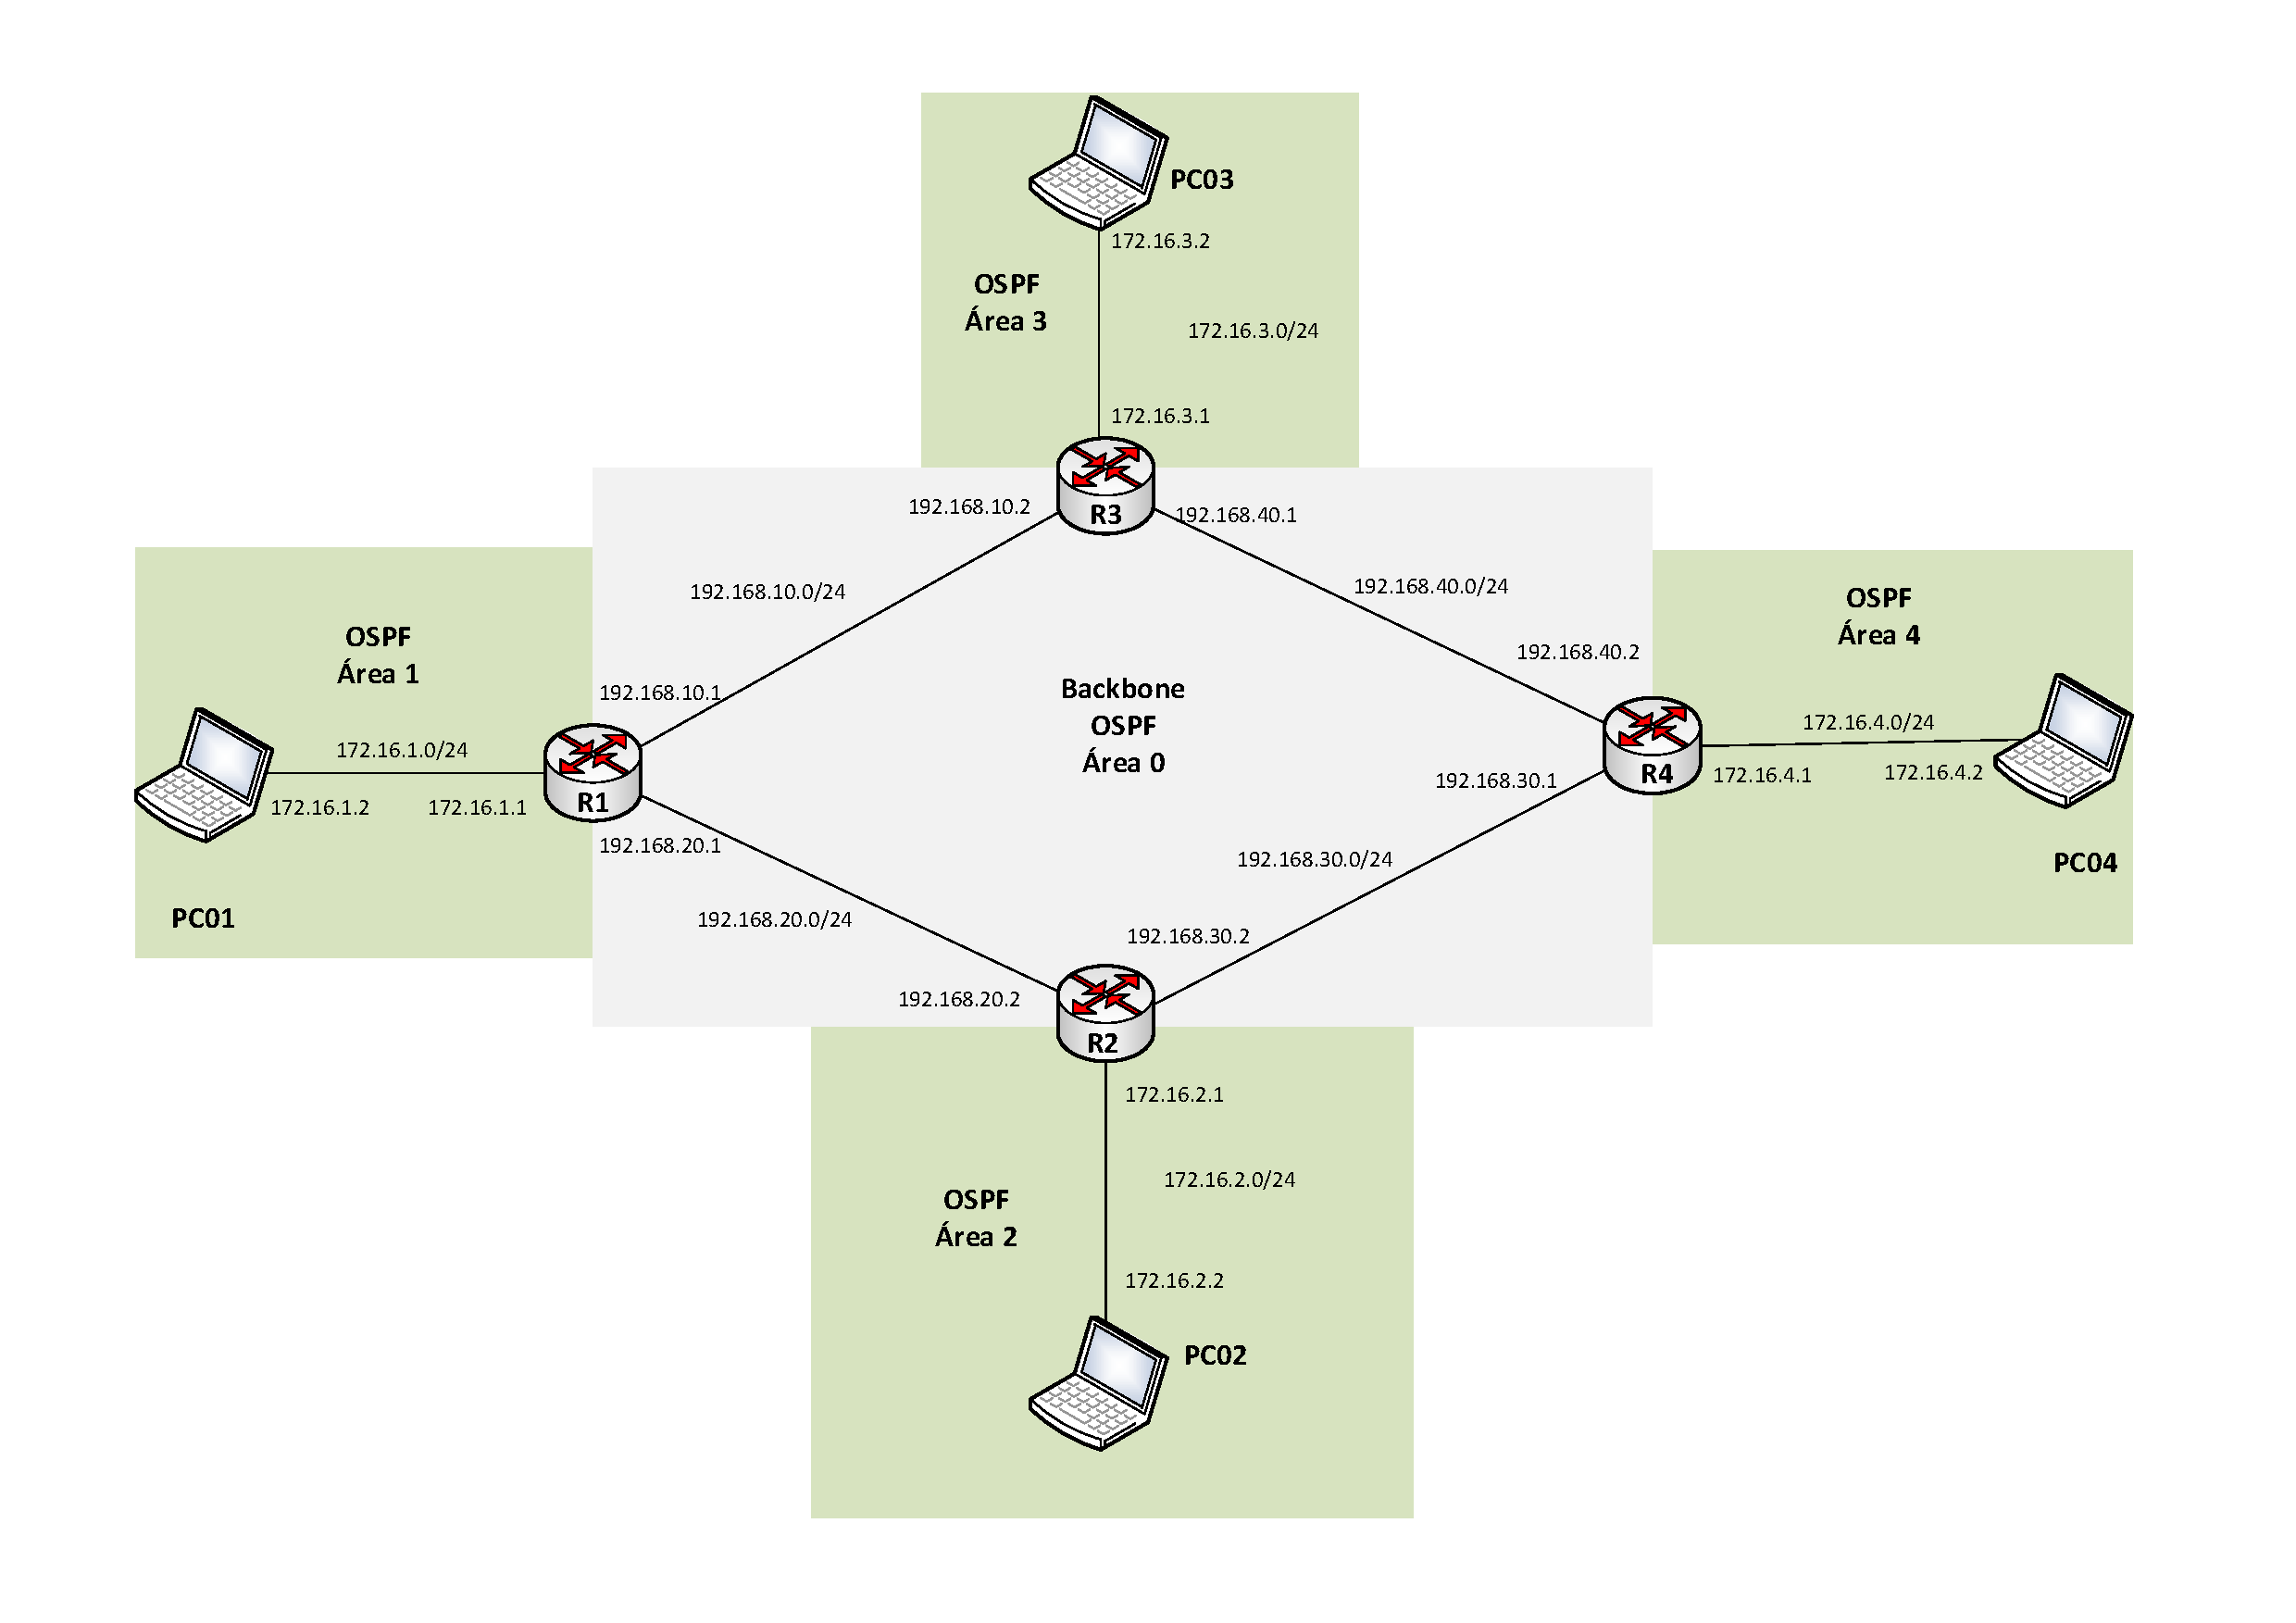
\includegraphics[width=\textwidth]{img/topologia-2.pdf}}    
        \end{figure}    
    \end{block}
\end{frame}

\section{Cronograma}

\subsection{Pendências}

\begin{frame}[fragile]{Cronograma}{Pendências}

    \begin{block}{Quagga}    
        \begin{itemize}
            \item Falta testar nos Raspberry;
            \item Falta interferir nas prioridades usando Python;
        \end{itemize}
    \end{block}

    \begin{block}{Decisão de roteamento}
        \begin{itemize}
            \item Algoritmo para decisão sobre quando mudar as prioridades
            \item Região de histerese para evitar "bouncing" de rotas
        \end{itemize}
    \end{block}
\end{frame}

\end{document}